\documentclass[aps,prl,reprint,notitlepage,nofootinbib,nobibnotes]{revtex4-2}

\usepackage[T1]{fontenc}
\usepackage{lmodern,microtype}
\usepackage{amsmath,amssymb,amsthm}
\usepackage{tikz}
\usetikzlibrary{arrows.meta,decorations.pathreplacing,calc}
\definecolor{FOneInk}{HTML}{293744}
\definecolor{FOneWire}{HTML}{A8B2BA}
\definecolor{FOneTeal}{HTML}{226E78}
\definecolor{FOneAmber}{HTML}{9D6826}
\definecolor{FOneNavy}{HTML}{3C496B}
\definecolor{LinkDarkRed}{HTML}{8B0000}
\usepackage{hyperref}
\hypersetup{
  colorlinks=true,
  allcolors=LinkDarkRed,
  citecolor=blue,
  urlcolor=blue,
  pdftitle={Finiteness of Shallow Logical Operators and a Sharp Depth Threshold},
  pdfsubject={All bounded-range logical circuits under a common total-depth bound}
}
\newtheorem{theorem}{Theorem}
\newtheorem{lemma}{Lemma}
\newcommand{\HH}{\mathcal H}
\newcommand{\UU}{\mathrm U}
\newcommand{\PU}{\mathrm{PU}}
\newcommand{\id}{I}
\newcommand{\tr}{\operatorname{Tr}}
\setlength{\emergencystretch}{0.7em}

\begin{document}
\title{Finiteness of Shallow Logical Operators and a Sharp Depth Threshold}
\author{Yimin Lu}
\email{lym23@mails.tsinghua.edu.cn}
\affiliation{Yau Mathematical Sciences Center, Tsinghua University, Beijing 100084, China\\
 Qiuzhen College, Tsinghua University, Beijing 100084, China}
\date{\today}

\begin{abstract}
For a quantum code on \(n\) finite-dimensional physical subsystems, we
consider all exact logical unitary circuits of depth at most \(h\ge1\), with
gates on at most \(\rho\) subsystems. For \(\rho\ge2\) and code distance
\(d\ge2\), these circuits have only finitely many logical actions, up to
phase, whenever \(h<2\lceil\log_{\rho} d\rceil-1\), where no stabilizer or geometric locality assumption is needed, and a gauge
subsystem is allowed. In contrast, for every qubit stabilizer code encoding at least one qubit, an infinite logical family is available at depth
\(2\lceil\log_{\rho} d\rceil-1\), for \(\rho\ge2\) and \(d\ge2\).
This is the exact critical depth for the onset of infinitely many
logical actions in that class.
\end{abstract}
\maketitle

During a quantum computation, circuit depth controls the spread of
physical errors. The gate range \(\rho\) is the maximum number of physical
subsystems on which an elementary gate may act. A single fault in a
depth-\(h\) circuit can affect at most \(\rho^h\) subsystems, so constant-depth
circuits of bounded range limit error propagation between
error-correction steps. Controlling this spread is central to
fault-tolerant computation. Under its code and decoding assumptions,
Gottesman's threshold construction protects polynomial-size
computations below a noise threshold with constant space
overhead~\cite{Gottesman}. We therefore ask which logical operations can
be realized at shallow depth and how much depth is needed for universal
logical control.

% TODO (author): Revise the background paragraph. Keep this marker for later review.
\textcolor{LinkDarkRed}{\textit{[To be revised.]}}\quad
Early Clifford-hierarchy bounds impose geometric or algebraic
assumptions beyond gate range and distance. Bravyi and K\"onig considered
local stabilizer checks and geometrically local gates~\cite{BK}.
Extensions to Pauli subsystem codes and geometrically nonlocal gates
use further cleaning or disjointness conditions~\cite{PY,JKY}.
Finiteness also appears for protected gates in two-dimensional
topological field theories~\cite{Beverland}, where equivalence can remove
separate phases on invariant sectors. Here only one global phase is
removed. Webster et al.\ restrict universal gate sets for
infinite-disjointness stabilizer-code families~\cite{Webster}, an
assumption not imposed here.

Under one common
total-depth bound, universal approximation requires infinitely many
exact logical actions. We therefore ask at what depth this
necessary condition can first hold. For \(\rho\ge2\) and \(d\ge2\),
Theorem~\ref{thm:depth} rules out an infinite logical image when
\(h<2\lceil\log_{\rho} d\rceil-1\), without a stabilizer or geometric locality
assumption. The finiteness criterion does not assign a Clifford
hierarchy level. Theorem~\ref{cor:critical} shows that every qubit stabilizer
subspace code encoding at least one qubit realizes a nontrivial
continuous logical family at depth \(2\lceil\log_{\rho} d\rceil-1\), when
arbitrary gates on at most \(\rho\) qubits are allowed. Stabilizer subspace
codes are thus the most capable base models for the onset of an infinite
logical family, attaining the smallest possible depth at given \(d\)
and \(\rho\).
Figure~\ref{fig:mechanisms} illustrates the two mechanisms.

\begin{figure*}[t]
\centering
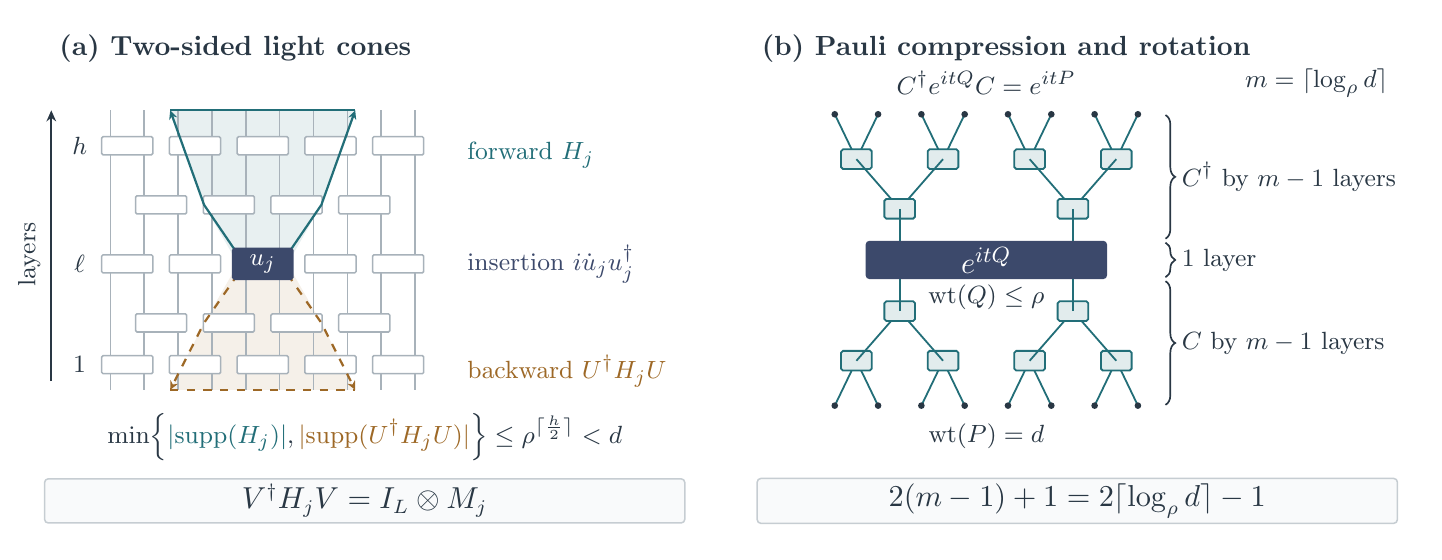
\begin{tikzpicture}[
 x=1cm,y=1cm,font=\fontsize{9.5}{11}\selectfont,text=FOneInk,
 f1wire/.style={draw=FOneWire,line width=0.55pt},
 f1brick/.style={draw=FOneWire,line width=0.55pt,fill=white,
   rounded corners=0.5pt},
 f1tree/.style={draw=FOneTeal,line width=0.65pt},
 f1clifford/.style={draw=FOneTeal,line width=0.65pt,
   fill=FOneTeal!13,rounded corners=0.7pt,
   minimum width=0.39cm,minimum height=0.25cm,inner sep=0pt},
 f1brace/.style={draw=FOneInk,line width=0.6pt,
   decorate,decoration={brace,amplitude=3.5pt}},
 f1footer/.style={draw=FOneWire!65,line width=0.55pt,
   fill=FOneNavy!3,rounded corners=1.3pt,minimum height=0.56cm,
   inner xsep=5pt,inner ysep=2pt},
 f1panel/.style={anchor=west,font=\bfseries\fontsize{10}{11.5}\selectfont}
]
\path[use as bounding box] (0,0) rectangle (17.6,6.4);
\node[f1panel] at (0.28,6.13) {(a) Two-sided light cones};
\node[f1panel] at (9.20,6.13) {(b) Pauli compression and rotation};

% (a) Gate insertion in a schematic circuit; time runs upward.
\path[fill=FOneTeal,fill opacity=0.10]
 (2.67,3.40)--(2.24,4.15)--(1.81,5.35)--(4.16,5.35)
 --(3.73,4.15)--(3.30,3.40)--cycle;
\path[fill=FOneAmber,fill opacity=0.10]
 (2.67,3.40)--(2.24,2.65)--(1.81,1.80)--(4.16,1.80)
 --(3.73,2.65)--(3.30,3.40)--cycle;
\foreach \i in {0,...,9}{
 \pgfmathsetmacro{\wx}{1.05+0.43*\i}
 \draw[f1wire] (\wx,1.80)--(\wx,5.35);
}
\foreach \yy in {2.12,3.40,4.90}{
 \foreach \i in {0,2,4,6,8}{
  \pgfmathsetmacro{\xa}{0.94+0.43*\i}
  \pgfmathsetmacro{\xb}{1.59+0.43*\i}
  \draw[f1brick] (\xa,\yy-0.115) rectangle (\xb,\yy+0.115);
 }
}
\foreach \yy in {2.65,4.15}{
 \foreach \i in {1,3,5,7}{
  \pgfmathsetmacro{\xa}{0.94+0.43*\i}
  \pgfmathsetmacro{\xb}{1.59+0.43*\i}
  \draw[f1brick] (\xa,\yy-0.115) rectangle (\xb,\yy+0.115);
 }
}
\draw[FOneTeal,line width=0.8pt,-{Stealth[length=3.2pt,width=3pt]}]
 (2.67,3.52)--(2.24,4.15)--(1.81,5.35);
\draw[FOneTeal,line width=0.8pt,-{Stealth[length=3.2pt,width=3pt]}]
 (3.30,3.52)--(3.73,4.15)--(4.16,5.35);
\draw[FOneTeal,line width=0.8pt] (1.81,5.35)--(4.16,5.35);
\draw[FOneAmber,line width=0.8pt,dashed,
 -{Stealth[length=3.2pt,width=3pt]}]
 (2.67,3.27)--(2.24,2.65)--(1.81,1.80);
\draw[FOneAmber,line width=0.8pt,dashed,
 -{Stealth[length=3.2pt,width=3pt]}]
 (3.30,3.27)--(3.73,2.65)--(4.16,1.80);
\draw[FOneAmber,line width=0.8pt,dashed] (1.81,1.80)--(4.16,1.80);
\node[draw=FOneNavy,fill=FOneNavy,text=white,line width=0.7pt,
 rounded corners=0.7pt,minimum width=0.76cm,minimum height=0.39cm,
 inner sep=0pt] at (2.985,3.40) {\(u_j\)};
\draw[FOneInk,line width=0.6pt,-{Stealth[length=4pt,width=3.5pt]}]
 (0.30,1.91)--(0.30,5.35);
\node[rotate=90,font=\fontsize{9}{10}\selectfont] at (0.02,3.52) {layers};
\node at (0.66,2.12) {\(1\)};
\node at (0.66,3.40) {\(\ell\)};
\node at (0.66,4.90) {\(h\)};
\node[anchor=west,align=left,text=FOneTeal] at (5.46,4.78)
 {forward \(H_j\)};
\node[anchor=west,align=left,text=FOneNavy] at (5.46,3.40)
 {insertion \(i\dot u_j u_j^\dagger\)};
\node[anchor=west,align=left,text=FOneAmber] at (5.46,2.04)
 {backward \(U^\dagger H_jU\)};
\node[inner sep=0pt] at (4.28,1.20)
 {\(\min\!\left\{
    \textcolor{FOneTeal}{\lvert\operatorname{supp}(H_j)\rvert},
    \textcolor{FOneAmber}{\lvert\operatorname{supp}(U^\dagger H_jU)\rvert}
   \right\}\le \rho^{\lceil \frac{h}{2}\rceil}<d\)};
\node[f1footer,minimum width=8.13cm,
 font=\fontsize{10.5}{12}\selectfont] at (4.28,0.39)
 {\(V^\dagger H_jV=I_L\otimes M_j\)};

% (b) Active Pauli support only. Binary branching illustrates the \rho-ary tree.
\node[anchor=east] at (17.40,5.70) {\(m=\lceil\log_{\rho} d\rceil\)};
\node at (12.175,5.70) {\(C^\dagger e^{itQ}C=e^{itP}\)};
\node at (12.175,1.21) {\(\operatorname{wt}(P)=d\)};
\foreach \sgn in {-1,1}{
 \pgfmathsetmacro{\yl}{3.45+\sgn*1.85}
 \pgfmathsetmacro{\yone}{3.45+\sgn*1.28}
 \pgfmathsetmacro{\ytwo}{3.45+\sgn*0.65}
 \pgfmathsetmacro{\yg}{3.45+\sgn*0.23}
 \foreach \xa/\xb/\xc in {
 10.25/10.80/10.525,11.35/11.90/11.625,
 12.45/13.00/12.725,13.55/14.10/13.825}{
  \draw[f1tree] (\xa,\yl)--(\xc,\yone);
  \draw[f1tree] (\xb,\yl)--(\xc,\yone);
  \node[f1clifford] at (\xc,\yone) {};
 }
 \foreach \xa/\xb/\xc in {10.525/11.625/11.075,12.725/13.825/13.275}{
  \draw[f1tree] (\xa,\yone)--(\xc,\ytwo);
  \draw[f1tree] (\xb,\yone)--(\xc,\ytwo);
  \node[f1clifford] at (\xc,\ytwo) {};
  \draw[f1tree] (\xc,\ytwo)--(\xc,\yg);
 }
 \foreach \xx in {10.25,10.80,11.35,11.90,12.45,13.00,13.55,14.10}{
  \fill[FOneInk] (\xx,\yl) circle (1.2pt);
 }
}
\node at (12.175,2.98) {\(\operatorname{wt}(Q)\le \rho\)};
\node[draw=FOneNavy,fill=FOneNavy,text=white,line width=0.7pt,
 rounded corners=1pt,minimum width=3.04cm,minimum height=0.46cm,
 inner sep=0pt,font=\fontsize{11}{12}\selectfont] at (12.175,3.45)
 {\(e^{itQ}\)};
\draw[f1brace] (14.45,3.18)--(14.45,1.61);
\node[anchor=west,align=left,inner xsep=0pt] at (14.65,2.395)
 {\(C\) by \(m-1\) layers};
\draw[f1brace] (14.45,3.67)--(14.45,3.23);
\node[anchor=west,inner xsep=0pt] at (14.65,3.45) {1 layer};
\draw[f1brace] (14.45,5.29)--(14.45,3.72);
\node[anchor=west,align=left,inner xsep=0pt] at (14.65,4.505)
 {\(C^\dagger\) by \(m-1\) layers};
\node[f1footer,minimum width=8.13cm,
 font=\fontsize{10.5}{12}\selectfont] at (13.33,0.39)
 {\(2(m-1)+1=2\lceil\log_{\rho} d\rceil-1\)};
\end{tikzpicture}
\caption{Mechanisms behind Theorems~\ref{thm:depth} and~\ref{cor:critical}.
Time runs upward in both panels.
(a) An insertion at gate \(u_j\) in layer \(\ell\) has forward and backward
supports bounded by \(\rho^{h-\ell+1}\) and \(\rho^\ell\).
When \(\rho^{\lceil \frac{h}{2}\rceil}<d\), at least one support is detectable.
The exact encoded action transfers its gauge-only compression to
\(V^\dagger H_jV=\id_L\otimes M_j\), for a gauge operator \(M_j\).
The brickwall arrangement is schematic and imposes no geometric locality.
(b) With \(m=\lceil\log_{\rho}d\rceil\) and \(\rho\ge2\), Clifford gates compress a
weight-\(d\) logical Pauli to \(Q=CPC^\dagger\) in \(m-1\) layers.
One gate \(e^{itQ}\) and \(m-1\) inverse layers give \(e^{itP}\) at depth
\(2m-1\). The case \((\rho,d)=(2,8)\) is illustrated. In general, a gate may collect
up to \(\rho\) factors. Only active Pauli support is shown. The physical qubits remain.}
\label{fig:mechanisms}
\end{figure*}

Let the physical system be \(\HH=\bigotimes_{i=1}^{n}\HH_i\), with
\(n\ge1\) and finite-dimensional factors. The code \(\mathcal C\) is specified
by an isometry \(V:\HH_L\otimes\HH_G\longrightarrow\HH\), where
\(\dim\HH_L=K\ge2\) and \(\dim\HH_G=g\ge1\). The factors carry logical and
gauge degrees of freedom, respectively.
A distance lower bound \(d\) means that every operator \(O\) supported on
fewer than \(d\) physical subsystems satisfies
\begin{equation}\label{eq:correctable}
  V^\dagger O V=\id_L\otimes M_O
\end{equation}
for some operator \(M_O\) on \(\HH_G\)~\cite{KL,Kribs}.
A physical unitary \(U\) implements an exact logical action when
\begin{equation}\label{eq:encoded}
  UV=V(W\otimes Z)
\end{equation}
for unitaries \(W\) on \(\HH_L\) and \(Z\) on \(\HH_G\).
This equality holds for all logical and gauge states, and the logical
action is the phase class \([W]\in\PU(K)\).
For integers \(h\ge1\) and \(\rho\ge2\), let
\(\mathcal L_{\le h}(\mathcal C,\rho)\) be the set of these classes obtained
when \(U\) has at most \(h\) layers of arbitrary unitary gates on disjoint
supports of at most \(\rho\) physical subsystems.
The depth bound applies to each complete circuit.

% TODO (author): Revise the methods paragraph. Keep this marker for later review.
\textcolor{LinkDarkRed}{\textit{[To be revised.]}}\quad
Eastin--Knill restricts transversal gates through a compact Lie-group
argument~\cite{EK}. Circuits subject to a common depth bound need not
form a group, and successive layers can have intersecting supports.
Our proof applies the infinitesimal restriction to circuit parameters
using both forward and backward light cones.
Detectable sums of generators on overlapping erasable regions have also
been studied in the theory of covariant error
correction~\cite{Faist,LiuZhou}. Polynomial circuit maps, their
conjugated gate-insertion derivatives, and semialgebraic stratification
are established tools in quantum circuit analysis~\cite{Haferkamp}.
The required code condition is error detection, allowing gauge degrees
of freedom~\cite{KL,Kribs}.
Our proof uses a finite smooth decomposition of a polynomial constraint
set~\cite{Plaumann}.

\begin{samepage}
\begin{theorem}\label{thm:depth}
Let \(n\ge1\), \(h\ge1\), and \(\rho\ge2\) be integers, and let
\(V\) encode a quantum code \(\mathcal C\) satisfying Eq.~\eqref{eq:correctable}
for an integer \(d\ge2\) on \(n\) physical subsystems. If
\begin{equation}\label{eq:depth}
  h<2\lceil\log_{\rho} d\rceil-1,
\end{equation}
then the logical actions of all circuits of depth at most \(h\), with gates
on at most \(\rho\) subsystems, that satisfy Eq.~\eqref{eq:encoded} obey
\[
 |\mathcal L_{\le h}(\mathcal C,\rho)|<\infty.
\]
All gate supports and unitary matrices are allowed. Consequently,
\(\mathcal L_{\le h}(\mathcal C,\rho)\) is not dense in \(\PU(K)\).
\end{theorem}
\end{samepage}

\begin{proof}
Equation~\eqref{eq:depth} is equivalent to
\(\rho^{\lceil \frac{h}{2}\rceil}<d\).

Group all circuits by the gate supports in each layer. After adding
singleton identity gates on idle sites, a layer is a partition of the
\(n\) sites into blocks of size at most \(\rho\). There are finitely many
such partitions, and hence finitely many support arrangements for \(h\)
layers. Circuits of smaller depth are included by identity padding.
The unitary matrices on these supports remain arbitrary.

Choose one arrangement, denoted by \(\alpha\), and list its gates in
layer order as \(u_1,\ldots,u_J\), so that \(U=u_J\cdots u_1\).
Consider a smooth family of gate matrices and logical factors \(W,Z\)
satisfying Eq.~\eqref{eq:encoded}. Its Hermitian generator is
\begin{equation}\label{eq:generator}
  H=i\dot U U^\dagger
   =\sum_{j=1}^{J}
      U_{>j}\bigl(i\dot u_j u_j^\dagger\bigr)U_{>j}^\dagger,
\end{equation}
where \(U_{>j}=u_J\cdots u_{j+1}\). This is the conjugated
gate-insertion derivative used in circuit parameter
analysis~\cite{Haferkamp}.
Write the \(j\)th summand as \(H_j\), and suppose that gate \(j\)
is in layer \(\ell\). Its forward light cone has at most
\(\rho^{h-\ell+1}\) sites. In the opposite frame,
\[
  U^\dagger H_jU
   =U_{<j}^\dagger(iu_j^\dagger\dot u_j)U_{<j},
\]
where \(U_{<j}=u_{j-1}\cdots u_1\). This operator has a backward
light cone of at most \(\rho^\ell\) sites. Other gates in layer \(\ell\)
have disjoint supports and cancel from both counts.
At least one of these two supports therefore has size at most
\[
  \rho^{\min\{\ell,h-\ell+1\}}
  \le \rho^{\lceil \frac{h}{2}\rceil}<d.
\]
If the forward support is smaller than \(d\),
Eq.~\eqref{eq:correctable} applies directly to \(H_j\).
If only the backward support is smaller, it gives
\(V^\dagger U^\dagger H_jUV=\id_L\otimes N_j\).
Equation~\eqref{eq:encoded} then implies
\begin{align*}
 V^\dagger H_jV
  &=(W\otimes Z)(\id_L\otimes N_j)(W^\dagger\otimes Z^\dagger)\\
  &=\id_L\otimes ZN_jZ^\dagger.
\end{align*}
Thus \(V^\dagger H_jV=\id_L\otimes M_j\) for every \(j\), with all
compressions taken in the same frame.
Summing gives
\begin{equation}\label{eq:compression}
  V^\dagger H V=\id_L\otimes M
\end{equation}
where \(M=\sum_{j=1}^{J}M_j\) is Hermitian on \(\HH_G\).
This is the detectable-generator step~\cite{EK,Faist}.

Differentiating Eq.~\eqref{eq:encoded}, and using
\(U^\dagger V=V(W^\dagger\otimes Z^\dagger)\), also gives
\begin{align}
  V^\dagger H V&=A\otimes\id_G+\id_L\otimes B,
       \label{eq:logicalgen}\\
  A&=i\dot W W^\dagger,\qquad B=i\dot Z Z^\dagger.\nonumber
\end{align}
Taking the partial trace over \(\HH_G\) yields
\[
  A=\frac{\tr(M-B)}{g}\,\id_L.
\]
Thus \(\dot W=-i\lambda W\) for a real scalar \(\lambda\), and the logical
motion is only a phase.

To obtain finiteness, let \(D_j\) be the Hilbert-space dimension on the
support of gate \(j\), and put
\[
  \mathcal P_\alpha=
  \left(\prod_{j=1}^{J}\UU(D_j)\right)
    \times\UU(K)\times\UU(g).
\]
Let \(\mathcal X_\alpha\subseteq\mathcal P_\alpha\) consist of the tuples
\((\mathbf u,W,Z)\) satisfying Eq.~\eqref{eq:encoded}.
Unitarity and Eq.~\eqref{eq:encoded} are polynomial equations in the real
and imaginary matrix entries, so \(\mathcal X_\alpha\) is a real algebraic
set.

Lemma~\ref{lem:finite-smooth-decomposition} in the End Matter gives
a finite smooth decomposition
\begin{equation}\label{eq:cells}
  \mathcal X_\alpha=\bigsqcup_{r=1}^{N_\alpha}C_r,
  \qquad N_\alpha<\infty,
\end{equation}
where each cell is smoothly diffeomorphic to an open cube
\((0,1)^{\nu_r}\), including a point when \(\nu_r=0\).
This partition also covers singular points of \(\mathcal X_\alpha\).

For two tuples \(x,y\in C_r\), choose a smooth diffeomorphism
\(\varphi_r:(0,1)^{\nu_r}\to C_r\), and set
\(a=\varphi_r^{-1}(x)\), \(b=\varphi_r^{-1}(y)\).
The path
\begin{equation}\label{eq:cellpath}
  \gamma(t)=\varphi_r\bigl((1-t)a+tb\bigr),
  \qquad 0\le t\le1,
\end{equation}
stays in \(C_r\). Its coordinates give smooth gate matrices and logical
factors satisfying Eq.~\eqref{eq:encoded} throughout.
The preceding calculation makes \([W]\) constant along \(\gamma\).
Each cell therefore contributes at most one logical operation modulo
phase, giving at most \(N_\alpha\) operations for this support arrangement.

The finitely many arrangements cover every circuit of depth at most \(h\)
and gate range at most \(\rho\). Thus
\(\mathcal L_{\le h}(\mathcal C,\rho)\) is a finite union of finite sets.
Since \(K\ge2\), it is closed and cannot be dense in \(\PU(K)\).
\end{proof}


Finiteness does not exclude a finite subset \(S\subseteq\mathcal L_{\le h}(\mathcal C,\rho)\)
for which
\[
 \overline{\langle S\rangle}=\PU(K).
\]
The group \(\langle S\rangle\) allows words of arbitrary finite length.
A word of length \(r\) in \(S\cup S^{-1}\) has a concatenated
implementation of depth at most \(rh\). These products are not required
to remain in \(\mathcal L_{\le h}(\mathcal C,\rho)\), so density of the generated group does not
assert density within the original depth bound.
For example, Dua et al.\ give a \([[37,1,7]]\) CSS code with separate depth-one
circuits of gate range \(\rho=3\) that
implement~\cite[Sec.~V and Appendix~B~3]{Dua}
\[
 S=\bigl\{\overline T^\dagger,
          \sqrt{\overline X}^{\,\dagger}\bigr\}
   \subseteq\mathcal L_{\le1}(\mathcal C,3).
\]
The two circuits use different partitions of the physical qubits.
Since \(\overline H\propto
(\overline T^\dagger)^2\sqrt{\overline X}^{\,\dagger}
(\overline T^\dagger)^2\) and
\(\overline T=(\overline T^\dagger)^7\), this pair generates a dense
subgroup of \(\PU(2)\). For this code,
\(2\lceil\log_3 7\rceil-1=3\), so \(\mathcal L_{\le1}(\mathcal C,3)\) is finite by
Theorem~\ref{thm:depth}.


In a fault-tolerance threshold construction based on the constant-depth
unitary logical gadgets considered here, logical-gate compilation is
necessary for universal control in the finite-image regime. On a fixed
code, the available shallow logical actions form a finite alphabet. If
its generated group is dense, arbitrary target logical unitaries can be
approximated by words over this alphabet, with error correction
interleaved as prescribed by the protocol~\cite{Gottesman,Dua}. The
constant-depth premise applies to each gadget. Compiled word lengths cannot
remain uniformly bounded when arbitrary targets must be approximated to
arbitrarily high accuracy.

The finiteness condition has an exact boundary for stabilizer codes. For an integer \(\rho\ge2\), define the critical depth
\begin{equation}\label{eq:critical-definition}
 h_\infty(\mathcal C,\rho)
  =\min\{h\in\mathbb Z_{\ge1}:\mathcal L_{\le h}(\mathcal C,\rho)
                   \text{ is infinite}\},
\end{equation}
with value \(\infty\) if the set is empty. For \(d\ge2\),
this definition and Theorem~\ref{thm:depth} give
\begin{equation}\label{eq:critical-lower}
 h_\infty(\mathcal C,\rho)\ge2\lceil\log_{\rho} d\rceil-1.
\end{equation}

The matching upper bound uses established Pauli-rotation synthesis.
Binary-tree compression appears in Ref.~\cite{BonetMonroig}, Sec.~IV and
Fig.~2(a). Cowtan et al.\ give balanced-tree phase gadgets with logarithmic
CNOT depth~\cite[Cor.~3.4 and the following discussion]{Cowtan}, and
Haah, Liu, and Tan explicitly obtain logarithmic-depth Pauli rotations
with all-to-all connectivity~\cite[Cor.~3.6]{HaahLiuTan}.
Choosing a weight-\(d\) logical Pauli gives the logarithmic upper bound
for stabilizer codes as a direct application. The depth-one
case with gate range at least \(d\) is also noted explicitly by
Dua et al.~\cite[Sec.~I]{Dua}, using a minimum-weight logical Pauli as
a rotation generator.

\begin{samepage}
\begin{theorem}\label{cor:critical}
Let \(\mathcal C\) be an \([[n,k,d]]\) qubit stabilizer code,
with \(k\ge1\) and actual distance \(d\ge2\). Let \(\rho\ge2\) be an
integer, and allow arbitrary unitary gates on any set of at most \(\rho\)
qubits. Then
\begin{equation}\label{eq:critical}
 h_\infty(\mathcal C,\rho)=2\lceil\log_{\rho} d\rceil-1.
\end{equation}
At this depth, the logical image contains a nontrivial continuous
one-parameter subgroup.
\end{theorem}
\end{samepage}

\begin{proof}
The lower bound is Eq.~\eqref{eq:critical-lower}. For a stabilizer code, the distance \(d\) is the minimum weight of a Hermitian
\(n\)-qubit Pauli operator that preserves the code space and acts
nonscalarly on it. Choose such an operator \(P\) of weight \(d\), with
\(P^2=\id\), and put \(m=\lceil\log_{\rho} d\rceil\).

Partition the nonidentity factors of \(P\) into groups of \(\rho\),
except possibly one smaller group.
On each group, basis changes and CNOTs conjugate the product to a Pauli
on one qubit. Their composition is a single allowed Clifford gate on
that group. The groups are disjoint, so these gates form one layer.
If \(w_r\) is the weight after \(r\) layers, then
\(w_{r+1}=\lceil \frac{w_r}{\rho}\rceil\) and \(w_0=d\), so
\(w_r=\lceil \frac{d}{\rho^r}\rceil\). Hence \(m-1\) layers give a Clifford circuit
\(C\) such that
\[
 Q=CPC^\dagger,\qquad \operatorname{wt}(Q)\le \rho.
\]
Local basis changes are included in the allowed Clifford gates and
require no additional layers. When \(m=1\), take \(C=\id\).
The family
\begin{equation}\label{eq:pauli-family}
 U(t)=C^\dagger e^{itQ}C=e^{itP}
\end{equation}
has depth at most \(2m-1\), since its middle factor is a single allowed
gate. It preserves the code and induces \(e^{it\overline P}\), where
\(\overline P\) is a nontrivial logical Pauli. Since \(\overline P\) has both eigenvalues \(\pm1\), these projective
actions have period \(\pi\) and form a nontrivial continuous
\(\mathrm U(1)\) subgroup.
\end{proof}

\begin{acknowledgments}
% Replace the placeholder below with the final acknowledgement.
\textit{Acknowledgement.}\quad[To be completed by the author.]
\end{acknowledgments}

\begin{thebibliography}{17}
\rightskip=0pt plus 1fil\relax
\bibitem{Gottesman}
D.~Gottesman,
\href{https://doi.org/10.26421/QIC14.15-16-5}
{Quantum Inf.\ Comput.\ \textbf{14}, 1338--1371 (2014)},
\href{https://arxiv.org/abs/1310.2984}{arXiv:1310.2984}.

\bibitem{BK}
S.~Bravyi and R.~K\"onig,
\href{https://doi.org/10.1103/PhysRevLett.110.170503}
{Phys.\ Rev.\ Lett.\ \textbf{110}, 170503 (2013)},
\href{https://arxiv.org/abs/1206.1609}{arXiv:1206.1609}.

\bibitem{PY}
F.~Pastawski and B.~Yoshida,
\href{https://doi.org/10.1103/PhysRevA.91.012305}
{Phys.\ Rev.\ A \textbf{91}, 012305 (2015)},
\href{https://arxiv.org/abs/1408.1720}{arXiv:1408.1720}.

\bibitem{JKY}
T.~Jochym-O'Connor, A.~Kubica, and T.~J.~Yoder,
\href{https://doi.org/10.1103/PhysRevX.8.021047}
{Phys.\ Rev.\ X \textbf{8}, 021047 (2018)},
\href{https://arxiv.org/abs/1710.07256}{arXiv:1710.07256}.

\bibitem{Beverland}
M.~E.~Beverland, O.~Buerschaper, R.~K\"onig, F.~Pastawski,
J.~Preskill, and S.~Sijher,
\href{https://doi.org/10.1063/1.4939783}
{J.\ Math.\ Phys.\ \textbf{57}, 022201 (2016)},
\href{https://arxiv.org/abs/1409.3898}{arXiv:1409.3898}.

\bibitem{Webster}
P.~Webster, M.~Vasmer, T.~R.~Scruby, and S.~D.~Bartlett,
\href{https://doi.org/10.1103/PhysRevResearch.4.013092}
{Phys.\ Rev.\ Research \textbf{4}, 013092 (2022)},
\href{https://arxiv.org/abs/2012.05260}{arXiv:2012.05260}.

\bibitem{KL}
E.~Knill and R.~Laflamme,
\href{https://doi.org/10.1103/PhysRevA.55.900}
{Phys.\ Rev.\ A \textbf{55}, 900 (1997)},
\href{https://arxiv.org/abs/quant-ph/9604034}{arXiv:quant-ph/9604034}.

\bibitem{Kribs}
D.~Kribs, R.~Laflamme, and D.~Poulin,
\href{https://doi.org/10.1103/PhysRevLett.94.180501}
{Phys.\ Rev.\ Lett.\ \textbf{94}, 180501 (2005)},
\href{https://arxiv.org/abs/quant-ph/0412076}{arXiv:quant-ph/0412076}.

\bibitem{EK}
B.~Eastin and E.~Knill,
\href{https://doi.org/10.1103/PhysRevLett.102.110502}
{Phys.\ Rev.\ Lett.\ \textbf{102}, 110502 (2009)},
\href{https://arxiv.org/abs/0811.4262}{arXiv:0811.4262}.

\bibitem{Faist}
P.~Faist, S.~Nezami, V.~V.~Albert, G.~Salton, F.~Pastawski,
P.~Hayden, and J.~Preskill,
\href{https://doi.org/10.1103/PhysRevX.10.041018}
{Phys.\ Rev.\ X \textbf{10}, 041018 (2020)},
\href{https://arxiv.org/abs/1902.07714}{arXiv:1902.07714}.

\bibitem{LiuZhou}
Z.-W.~Liu and S.~Zhou,
\href{https://doi.org/10.1038/s41534-023-00788-4}
{npj Quantum Inf.\ \textbf{9}, 119 (2023)},
\href{https://arxiv.org/abs/2111.06355}{arXiv:2111.06355}.
See also its long supplement,
\href{https://arxiv.org/abs/2111.06360}{arXiv:2111.06360}, Sec.~VI.

\bibitem{Haferkamp}
J.~Haferkamp, P.~Faist, N.~B.~T.~Kothakonda, J.~Eisert, and
N.~Yunger~Halpern,
\href{https://doi.org/10.1038/s41567-022-01539-6}
{Nat.\ Phys.\ \textbf{18}, 528 (2022)},
\href{https://arxiv.org/abs/2106.05305}{arXiv:2106.05305},
Methods and Appendix~A.

\bibitem{Plaumann}
D.~Plaumann,
\href{https://wwwold.mathematik.tu-dortmund.de/~dplauman/notes/rag-ihp.pdf}
{\emph{Real Algebraic Geometry}}
(IHP lecture notes, 2023), Cor.~8.4 and the following discussion.

\bibitem{Dua}
A.~Dua, A.~Holmes, M.~J.~Gullans, and V.~V.~Albert,
\emph{Qubit CSS codes with Universal Transversal Gates},
\href{https://arxiv.org/abs/2610.06730v1}{arXiv:2610.06730v1} (2026).
\bibitem{BonetMonroig}
X.~Bonet-Monroig, R.~Sagastizabal, M.~Singh, and T.~E.~O'Brien,
\href{https://doi.org/10.1103/PhysRevA.98.062339}
{Phys.\ Rev.\ A \textbf{98}, 062339 (2018)},
\href{https://arxiv.org/abs/1807.10050}{arXiv:1807.10050}.

\bibitem{Cowtan}
A.~Cowtan, S.~Dilkes, R.~Duncan, W.~Simmons, and S.~Sivarajah,
\href{https://doi.org/10.4204/EPTCS.318.13}
{Electron.\ Proc.\ Theor.\ Comput.\ Sci.\ \textbf{318}, 213 (2020)},
\href{https://arxiv.org/abs/1906.01734}{arXiv:1906.01734}.

\bibitem{HaahLiuTan}
J.~Haah, Y.~Liu, and X.~Tan,
\href{https://doi.org/10.1007/s00220-025-05480-6}
{Commun.\ Math.\ Phys.\ \textbf{406}, 309 (2025)},
\href{https://arxiv.org/abs/2402.05239}{arXiv:2402.05239}.

\end{thebibliography}

\section*{End Matter}
\subsection*{Finite smooth decomposition of polynomial zero sets}

Together with the infinitesimal argument of Theorem~\ref{thm:depth},
finite Whitney stratification of the semialgebraic constraint set into
connected smooth strata already gives a finite logical image.
To keep the argument elementary and self-contained, we give a short proof
using linear algebra and the implicit function theorem, with elementary
polynomial arithmetic. The finite decomposition below is the polynomial
case of standard semialgebraic theory~\cite{Plaumann}.
A smooth cell below means an
embedded smooth submanifold that is smoothly diffeomorphic to an open
cube \((0,1)^r\), with a point allowed
when \(r=0\). No smoothness of the full zero set is assumed.

\begin{lemma}\label{lem:finite-smooth-decomposition}
For any finite family of real polynomials on \(\mathbb R^N\), there is a
finite partition of \(\mathbb R^N\) into smooth cells on each of which
every polynomial has constant sign. Consequently, the common zero set
of finitely many real polynomials is a finite disjoint union of smooth
cells.
\end{lemma}

\begin{proof}
We induct on \(N\). In one variable, the finitely many real roots of
the nonzero polynomials partition the line into points and open
intervals. The assertion is also immediate for \(N=0\).
Write the variables in the induction step as \((x,t)\), where
\(x\in\mathbb R^{N-1}\). Discard identically zero input polynomials,
and write the remaining ones as \(p_1(x,t),\ldots,p_a(x,t)\).

We first specify a finite family of projection polynomials in \(x\).
For every nonempty subset \(I\subseteq\{1,\ldots,a\}\), form
\(F_I=\prod_{i\in I}p_i\) and include all its coefficients in \(t\).
For every truncation
\[
 f(x,t)=\sum_{j=0}^{m}f_j(x)t^j
\]
of \(F_I\), with \(1\le m\le\deg_t F_I\), also include all square
minors of the coefficient matrix of the linear map
\begin{equation}\label{eq:endmatter-Sylvester}
 \begin{gathered}
 T_f:(A,B)\longmapsto Af+B\partial_t f,\\
 \deg A\le m-1,\qquad\deg B\le m.
 \end{gathered}
\end{equation}
The target consists of polynomials of degree at most \(2m-1\), so this
matrix has \(2m\) rows and \(2m+1\) columns. Its entries and minors are
polynomials in \(x\). Zero polynomials may be discarded. There are
finitely many subsets, truncations, coefficients, and minors.
By induction, partition the base \(\mathbb R^{N-1}\) into finitely many
smooth cells on which these projection polynomials have constant signs.

Fix one base cell \(C\). Each \(p_i\) is either identically zero as a
polynomial in \(t\) at every \(x\in C\), or has one constant degree
there. This follows from the coefficient signs. If all are identically
zero, the cylinder \(C\times\mathbb R\) is already a suitable cell.
Otherwise let \(I\) be the indices of the nonzero factors and set
\(F=F_I\). Its degree \(m\) is constant on \(C\). If \(m=0\), the same
cylinder suffices. Suppose \(m\ge1\). The truncation at this degree
agrees with \(F\) on every fiber over \(C\), so its projected matrix
represents \(T_F\).

The projected minors make the rank of \(T_F\) constant on \(C\).
At a point \(x\), write
\(F=d_0 f_0\), \(\partial_tF=d_0 g_0\), where \(d_0\) is the monic greatest
common divisor and \(f_0,g_0\) are coprime. Put \(s=\deg d_0\) and
\(r=m-s\). Then \(\deg f_0=r\), \(\deg g_0=r-1\), and \(r\ge1\).
The identity \(AF+B\partial_tF=0\) holds exactly when
\(A=Qg_0\) and \(B=-Qf_0\). The degree restrictions in
Eq.~\eqref{eq:endmatter-Sylvester} give \(\deg Q\le s\). Hence
\[
 \dim\ker T_F=s+1,\qquad \operatorname{rank}T_F=2m-s.
\]
In particular, \(s\) and \(r\) are constant on \(C\).

The monic squarefree part \(G=\frac{f_0}{c}\), where \(c\) is the leading
coefficient of \(F\), has precisely the real roots of \(F\), each
simple: differentiation lowers each root multiplicity by one.
We show that its coefficients depend smoothly on \(x\in C\), even
where \(F\) has repeated roots. Solve
\begin{equation}\label{eq:endmatter-monic-kernel}
 \begin{gathered}
 AF+B\partial_tF=0,\qquad\deg A<r,\\
 B=t^r+\sum_{j<r}b_jt^j.
 \end{gathered}
\end{equation}
There is exactly one solution: \(A=-\frac{g_0}{c}\), \(B=\frac{f_0}{c}\). The coefficient
matrix for the \(2r\) unknown coefficients is a column submatrix of
\(T_F\). It has full column rank: a homogeneous
solution would have \(\deg B<r\), whereas any nonzero kernel vector
has \(B=-Qf_0\) of degree at least \(r\).
Choose a nonzero \(2r\)-by-\(2r\) minor of this coefficient matrix
at one point of \(C\). It is among
the projected minors and thus remains nonzero throughout \(C\).
Cramer's rule expresses every coefficient in Eq.~\eqref{eq:endmatter-monic-kernel}
as a rational function of \(x\) with a denominator that does not vanish
on \(C\). Thus \(G=B\), the monic squarefree part, has smooth
coefficients on \(C\). The same construction for the singleton
products gives a smooth monic squarefree part \(G_i\) for every
nonconstant active factor \(p_i\).

The number of real roots of \(G\) is locally constant on \(C\).
Indeed, at a point \(x_0\), its real roots are simple. Apply the
implicit function theorem in a smooth coordinate chart of \(C\):
each root persists uniquely and smoothly. A monic
polynomial \(t^r+\sum_{j<r}b_jt^j\) has all its real roots in
\(\lvert t\rvert\le1+\max_j\lvert b_j\rvert\). Near \(x_0\), this
gives one uniform bound. Outside small disjoint intervals about the old
roots, \(G(x_0,t)\) is bounded away from zero on the remaining compact
interval. Continuity excludes new roots there. Within the small
intervals, the derivative stays nonzero and there is exactly one root.
Since \(C\) is connected, the number of real roots is constant, and
ordering them gives globally smooth functions
\[
 \theta_1(x)<\cdots<\theta_b(x).
\]

Inactive factors vanish identically, and active constant factors have
constant nonzero signs. For an active nonconstant factor, suppose
\(p_i(x_0,\theta_j(x_0))=0\).
The simple root of \(G_i\) at that point persists as a smooth root
\(\beta(x)\). Because \(p_i\) divides \(F\), this is also a root of
\(G\), and the local uniqueness of the latter root gives
\(\beta(x)=\theta_j(x)\). Thus vanishing on the graph is an open
condition in \(C\). Nonvanishing is open by continuity. Connectedness
makes one alternative hold everywhere, and any nonzero sign is then
constant.

Partition \(C\times\mathbb R\) into these \(b\) root graphs and the
\(b+1\) intervening open bands, including the unbounded bands.
No active factor vanishes in a band, so its sign is constant there.
A graph is diffeomorphic to \(C\). A band is diffeomorphic to
\(C\times(0,1)\). For finite endpoints use affine interpolation.
For a half-line use \(\frac{u}{1-u}\), and for the whole line use
\(\frac{u}{1-u}-\frac{1-u}{u}\), where \(0<u<1\).
Thus all pieces are smooth cells. There are finitely many base cells,
and each yields finitely many pieces. This completes the induction. The common zero set is the union of those cells on which
all the given polynomials vanish.
\end{proof}

This construction includes nullified factors, degree drops, repeated
roots, and singular points of the zero set. The subset products handle
factors that vanish on a base cell. The truncations handle degree drops.
The projected minors separate rank changes. Nothing requires the
polynomial zero set itself to be a manifold.

To apply the lemma, express the unitary and encoding constraints
for one circuit-support arrangement in real and imaginary matrix
entries. Their common zero set is \(\mathcal X_\alpha\).
For two points in one cell, a smooth chart from an open cube carries
the straight segment between their preimages to a smooth path in
\(\mathcal X_\alpha\). The circuit calculation in Theorem~\ref{thm:depth}
gives \(\dot W=-i\lambda W\) along this path, so its endpoints have the
same projective logical action. Each cell contributes at most one such
action. Finitely many cells, followed by finitely many support
arrangements, give the claimed finiteness.

\end{document}
